\documentclass[12pt, titlepage]{article}

\usepackage{booktabs}
\usepackage{tabularx}
\usepackage{hyperref}
\usepackage{float}
\usepackage{graphicx}
\hypersetup{
    colorlinks,
    citecolor=blue,
    filecolor=black,
    linkcolor=red,
    urlcolor=blue
}

%% Comments

\usepackage{color}

\newif\ifcomments\commentstrue %displays comments
%\newif\ifcomments\commentsfalse %so that comments do not display

\ifcomments
\newcommand{\authornote}[3]{\textcolor{#1}{[#3 ---#2]}}
\newcommand{\todo}[1]{\textcolor{red}{[TODO: #1]}}
\else
\newcommand{\authornote}[3]{}
\newcommand{\todo}[1]{}
\fi

\newcommand{\wss}[1]{\authornote{magenta}{SS}{#1}} 
\newcommand{\plt}[1]{\authornote{cyan}{TPLT}{#1}} %For explanation of the template
\newcommand{\an}[1]{\authornote{cyan}{Author}{#1}}

%% Common Parts

\newcommand{\progname}{ProgName} % PUT YOUR PROGRAM NAME HERE
\newcommand{\authname}{Team \#, Team Name
\\ Student 1 name
\\ Student 2 name
\\ Student 3 name
\\ Student 4 name} % AUTHOR NAMES                  

\usepackage{hyperref}
    \hypersetup{colorlinks=true, linkcolor=blue, citecolor=blue, filecolor=blue,
                urlcolor=blue, unicode=false}
    \urlstyle{same}
                                


\begin{document}

\title{System Verification and Validation Plan for \progname{}} 
\author{\authname}
\date{\today}
	
\maketitle

\pagenumbering{roman}

\section*{Revision History}

\begin{tabularx}{\textwidth}{p{3cm}p{2cm}X}
\toprule {\bf Date} & {\bf Version}\\
\midrule
All & 1.0\\
\bottomrule
\end{tabularx}

\newpage

\tableofcontents

\section{Symbols, Abbreviations, and Acronyms}

symbol description

T Test

This document will cover our team’s plan to ensure our project will do what we intend it to do, and will meet our stakeholders’ needs. This will cover background information regarding our software project and team, high--level plans for verifying all of the important artifacts of our project, detailed descriptions of system and unit tests, and lastly, a list of usability survey questions.

\section{General Information}

This section covers key background information related to the project.

\subsection{Summary}

The software being tested is our game, Ad Natura. This 2D pixel art styled puzzle platformer will take a player on a short adventure through a few levels with environmental puzzles to solve. Two key functions that will be the subject of much verification and validation testing will be the function of destroying and decomposing terrain into small pixel chunks, and the function of the slime mold organism traversing through the area and reacting to environmental stimuli.

\subsection{Objectives}

\begin{itemize}
  \item This project’s key objectives include:
\end{itemize}

Establish confidence in software correctness for the primary two functions: Terrain decomposition and the slime mold organism.

Establish confidence in software safety and security.

Demonstrate our message of cooperation between humans and nature, through the use of aesthetics and environmental storytelling.

Demonstrate satisfactory usability for both gamers and non--gamers, to expand to a wide audience.

\begin{itemize}
  \item Objectives that are out of scope for this project include:
\end{itemize}

Establishing confidence in software correctness for fundamental Unity engine code and functions. This is not necessary as we can assume that Unity’s engine has been thoroughly verified.

Demonstrating eye--catching, memorable visuals and music. These aspects are only important for marketing purposes, which is a very late--stage concern, and therefore not within the scope of this project at this stage.

\subsection{Extras}

The extras include a Design Thinking Report and a Usability Report. The Design Thinking Report will demonstrate the iterative design process, showing our work at each stage of development, and the reasoning behind each important decision we made. The Usability Report will take data collected from stakeholder testers to assess the usability of our system and determine any potential improvements that could be made.

\subsection{Relevant Documentation}

\begin{itemize}
  \item Relevant documents include:
\end{itemize}

Problem Statement and Goals. This document includes information about our goals, which is what the Verification and Validation Plan’s objectives are based on. It also lists stakeholders, which are relevant to our testing efforts.

Development Plan. This document describes our plan for our Proof of Concept Demonstration, which again highlights our most important objectives.

Software Requirements Specification. This document details all of the requirements, most of which will be subject to verification.

Hazard Analysis. This document includes some safety and security focused software requirements, which will be subject to verification.

Module Guide. This document describes all of the modules of our system. This is important for organizing our System and Unit Tests.

Module Interface Specification. This document describes specifications for the interfaces. This is also important for organizing our System and Unit Tests.

\section{Plan}

\subsection{Verification and Validation Team}

Todo: add another column for primary document, maybe another column for secondary, add other column as role (author/supervisor)

\subsection{SRS Verification}

We intend to use a mix of ad hoc feedback from fellow team members and our supervisor, and a proper structured plan. This will be done via a structured inspection process involving both internal team reviews and external stakeholder feedback. Internally, team members will use an ad hoc feedback approach to log any issues concerning clarity or consistency in our central issue tracker. For our supervisor, we will conduct a formal meeting where we present the game concept and critical requirements, followed by a Task--Based Inspection. The supervisor will be asked to specifically review pre--selected, complex requirements related to environment manipulation, physics simulations, and various elements of our project, such as the slime mold algorithm that we are using, focusing on their feasibility and testability. This ensures a structured approach to leveraging our supervisor's expertise beyond a simple read--over.

\subsection{Design Verification}

Our design verification plan focuses on ensuring the architectural and detailed design correctly implements the SRS and follows good software engineering principles like modularity. The core of this verification will be formal design inspections and walk--throughs. The Lead Developer will walk the team and classmates through critical design elements, such as the Tool--Effect System Architecture and the Level Data Structure, to scrutinize interface specifications and component interactions. Classmates will be leveraged as peer reviewers to ensure the design is robust and maintainable. The review process will focus on whether the design efficiently supports all functional requirements for traversing and manipulating the puzzle environments.

\subsection{Verification and Validation Plan Verification}

We will subject this document to a formal peer review by classmates, ensuring the plan adequately covers verification for all key project artifacts (SRS, Design, Implementation) and specifies a viable strategy for testing and validation. Additionally, we will employ conceptual mutation testing by deliberately considering how the plan would handle various types of software failures (e.g., unit test failure, non--functional requirement breach). We will also be subject to a review by Dr. Kelley and Michelle Bunton, to ensure that the core ideas and themes of the game, which may not be understood by classmates, are conveyed properly and free from errors in the document, as well as proper testing mechanisms for aspects which cannot be unit tested, like slime mold algorithm.

TODO: add explanation/hyperlink once, and then refer back to explanation for confusing elements such as SMA (best done when transferring to latex)

\subsection{Implementation Verification}

This verification relies heavily on three components: automated testing, manual testing, and static analysis. We will execute all automated tests detailed in the Unit Testing Plan, covering critical logic like physics calculations and tool--effect application, that can be mathematically verified. For static verification, the team will conduct internal code inspections on complex components, such as the logic for object mutation. Furthermore, the final presentation in CAS 741 will be used as both a formal Code Walk--Through and to help with one of our extras which was a usability report, where a section of the most complex game logic is presented and explained to an external audience, and a usability survey can also be conducted. For manual tests (integration testing), we need to ensure that the game components connect well, and that the goals we set are being met such as framerate, graphics, tools working properly under different conditions, etc.

\subsection{Automated Testing and Verification Tools}

We will use a unit testing framework such as xUnit or NUnit to test the parts of our code that can be tested via unit testing, such as physics calculations. We will also use a linter to ensure coding standards according to the coding standards described in the development plan. We will also use open source code coverage tools to determine the coverage of our tests, and highlight where we need to focus our efforts. We may use Continuous Integration to ensure all current code with tests is constantly passing the tests.

\subsection{Software Validation}

We will use the Rev 0 demo to our supervisor/stakeholder as the first key opportunity for requirements validation, ensuring the core mechanics align with their expectations. If we are able to, we will also be demoing to a small group of external user testers, likely our friends or classmates in engineering programs, that can provide us with feedback. These users will be engaged in task--based inspection, where they are asked to complete specific puzzle levels while being observed. Feedback will be gathered on the usability of the tool--selection interface and the satisfaction of the core puzzle loop, directly validating the non--functional and game design requirements. We will then ask them questions based on their experience, and seeing what aspects they enjoyed or did not enjoy, and what they found easy or difficult to use.

\section{System Tests}

System tests provide an effective and quantifiable way of evaluating success of functional and non--functional requirements.

-- When you talk about a survey/questionnaire, reference the Appendix.

\subsection{Tests for Functional Requirements}

The following are tests for the functional requirements outlined in the SRS.

Testing for functional requirements will include the two key game mechanics of destructive environment and path traversal as well as the saving feature. Each feature and mechanics’ specific functionalities will be tested to ensure it meets proper adherence to functionality.

\subsubsection{Saving Feature}

Outlined here are the required tests for the saving mechanic.

\subsubsection{FRT01}

\textbf{Control}: Manual\\
\textbf{Initial State}: Character at beginning of level.\\
\textbf{Input}: Move character to designated save point, destroy 2 objects, clicks save.\\
\textbf{Output}: Character coordinates, inventory, attributes, world state and game objects, and location saved to file.\\
\textbf{Test Case Derivation}: The saved information represents a snapshot of the player character to be loaded again to continue where the player has been left off.\\
\textbf{How test will be performed}: The user will move the character from point A to point B and perform the intended environmental manipulation and then click save.  The user loads the game save and checks if the current state is maintained.\\
\subsubsection{FRT02}

\textbf{Control}: Manual\\
\textbf{Initial State}: Character at beginning of level.\\
\textbf{Input}: Picks up 2 objects which will trigger save.\\
\textbf{Output}: Character coordinates, inventory, attributes, world state and game objects and location saved to file.\\
\textbf{Test Case Derivation}: The saved information represents a snapshot of the player character to be loaded again to continue where the player has been left off.\\
\textbf{How the test will be performed}: User will move the character from point A to point B and pick up the designated objects which will trigger save.  The user loads the game save and checks if the current state is maintained.\\
\subsubsection{Destructible Environment}

Outlined here are the required tests for the destructible environment mechanic.

\subsubsection{FRT03}

\textbf{Control}: Manual\\
\textbf{Initial State}: Character at beginning of level\\
\textbf{Input}: Go to designated point and use tool to destroy object at marked entry point. Repeat process with each tool and 3 different object attributes(soft object, brittle object, and hard object).\\
\textbf{Output}: Deformed original game object and spawned debris objects\\
\textbf{Test Case Derivation}: The deformed original game objects as well as the spawned game objects display shape deformation characteristics of the tool used and object attributes.\\
\textbf{How the test will be performed}: User will move the character to designated point and use tool to destroy object at marked entry point. Repeat process with each tool and 3 different object attributes(soft object, brittle object, and hard object.\\
\subsubsection{Slime Mold}

Outlined here are the required tests for the destructible environment mechanic.

\subsubsection{FRT04}

\textbf{Control}: Automatic\\
\textbf{Initial State}: Slime mold at spawned point, water debris at spawned point. 5 rectangular obstacles in the level each varying in size and dimensions, and one gap in terrain.\\
\textbf{Input}: Default slime mold entity spawn.\\
\textbf{Output}: Slime mold segments traverse to the water debris through the obstacles.\\
\textbf{Test Case Derivation}: Slime mold segments should travel from start to water debris objective in different and non deterministic ways each time in such the pathways traversed will be unique.\\
\textbf{How test will be performed}: Level will be set up with the game objects with  the specified initial state and the slime mold will traverse to the water debris. Screenshot taken of each run of the experiment.\\
...

\subsection{Tests for Nonfunctional Requirements}

The following are tests for the nonfunctional requirements outlined in the SRS.

\subsubsection{Save Game}

Outlined here are the required tests for the saving mechanic.

\subsubsection{NFRT01}

\textbf{Type}: Non--Functional\\
\textbf{Initial State}: Game Saved to file.\\
\textbf{Input/Condition}: run save file through decompression and deserialization check.\\
\textbf{Output/Result}: Console logged logical checks for each aspect of save file(player location, inventory, state, world object locations, etc)\\
\textbf{How test will be performed}: At a given point midway through a level, player will save the game, the save file with be run through our decompression and deserialization check and be evaluated if it passes all the logical checks\\
\subsubsection{Destructible Environment}

Outlined here are the required tests for the saving mechanic.

\subsubsection{NFRT02}

\textbf{Type}: Non--Functional\\
\textbf{Initial State}: Isolated Segments of levels, whole levels\\
\textbf{Input}: In the given test environment, the player will traverse from point A to B and is required to destroy certain terrain and objects between the traversal.\\
\textbf{Output}: Final game objects and terrain shape, generated debris, player traversal from point A to B\\
\textbf{How test will be performed}: In the given test environment setup to test critical sections of levels, the player will traverse from point A to B and is required to destroy certain terrain and objects between the traversal. Player actions are observed and are requested to fill out a survey (part of Section 6) with questions about traversability, issues with level design and destruction mechanics\\
\subsubsection{Slime Mold Algorithm Test}

Outlined here are the required tests for the saving mechanic.

\subsubsection{NFRT03}

\textbf{Type}: Non--Functional\\
\textbf{Initial State}: Slime mold at spawned point, water debris at spawned point. Obstacles in level 5 varying in size and width boxes, and one gap in terrain.\\
\textbf{Input}: N/A\\
\textbf{Output}: Slime mold traversal from spawned point to desired end point, Screenshot of final result.\\
\textbf{How test will be performed}: 3 Trials will be conducted with the same test level. Observations on traversability, randomness, and evaluation comments will be made in a survey(part of section 6) by the developer.\\
\subsection{Traceability Between Test Cases and Requirements}

The following is a table for the test cases as the relate to the requirements

\section{Unit Test Description}

\subsection{Unit Testing Scope}

\subsection{Tests for Functional Requirements}

\subsubsection{Module 1}

1. test--id1

\textbf{Type}: [Functional, Dynamic, Manual, Automatic, Static etc. Most will be automatic —SS]\\
\begin{itemize}
  \item Initial State:
  \item Input:
\end{itemize}

\textbf{Output}: [The expected result for the given inputs —SS]\\
\textbf{Test Case Derivation}: [Justify the expected value given in the Output field —SS]\\
\begin{itemize}
  \item How test will be performed:
\end{itemize}

2. test--id2

\textbf{Type}: [Functional, Dynamic, Manual, Automatic, Static etc. Most will be automatic —SS]\\
\begin{itemize}
  \item Initial State:
  \item Input:
\end{itemize}

\textbf{Output}: [The expected result for the given inputs —SS]\\
\textbf{Test Case Derivation}: [Justify the expected value given in the Output field —SS]\\
\begin{itemize}
  \item How test will be performed:
\end{itemize}

3. ...

\subsubsection{Module 2}

...

\subsection{Tests for Nonfunctional Requirements}

\subsubsection{Module ?}

1. test--id1

\textbf{Type}: [Functional, Dynamic, Manual, Automatic, Static etc. Most will be automatic —SS]\\
\begin{itemize}
  \item Initial State:
  \item Input/Condition:
  \item Output/Result:
  \item How test will be performed:
\end{itemize}

2. test--id2

\textbf{Type}: Functional, Dynamic, Manual, Static etc.\\
\begin{itemize}
  \item Initial State:
  \item Input:
  \item Output:
\end{itemize}

\textbf{How test will be performed}: \\
\subsubsection{Module ?}

...

\subsection{Traceability Between Test Cases and Modules [Provide evidence that all of the modules have been considered. —SS]}

References

Author Author. System requirements specification. https://github.com/..., 2019.

\section{Appendix}

This is where you can place additional information.

\subsection{Symbolic Parameters}

The definition of the test cases will call for SYMBOLIC CONSTANTS. Their values are defined in this section for easy maintenance.

The following symbolic constants are referenced by system and non--functional tests (Sec. 4). Centralizing them here keeps test cases consistent if values change.

\begin{figure}[H]
\centering
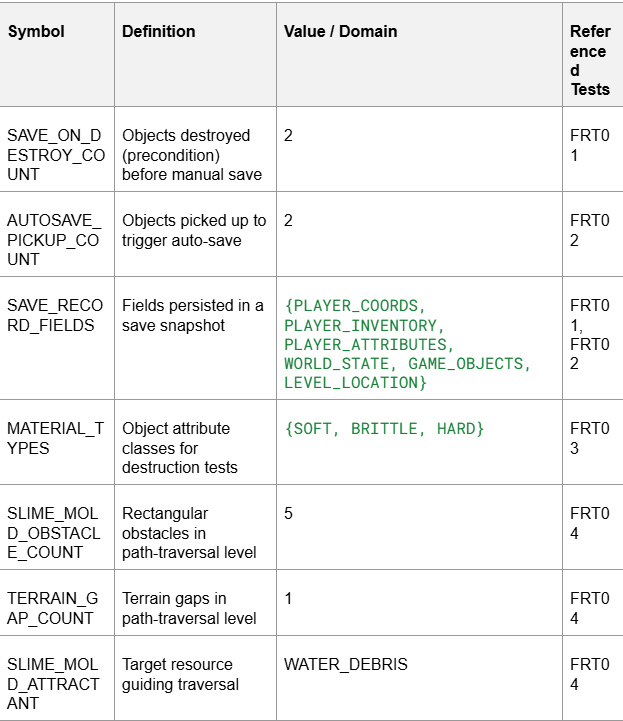
\includegraphics[width=\linewidth, height=0.8\textheight, keepaspectratio]{table.png}
\caption{Symbolic Parameters}
\label{tab:symbolic--parameters}
\end{figure}




Notes: SAVE\_RECORD\_FIELDS mirrors the save--snapshot contents described in the save tests; “LEVEL\_LOCATION” denotes the level/area identifier distinct from PLAYER\_COORDS.

\subsection{Usability Survey Questions}

\subsubsection{Operational Definitions}

• Fairness (puzzles): The reason for failure/success is understandable; rules/hints are telegraphed; no pixel--perfect timing is required; a recovery path exists.

• Soft--lock: Progress cannot be made without a menu reset or hard restart. Recovering within $\leq$60 s using in--game options does not count as a soft--lock.

\subsubsection{Purpose}

This survey evaluates whether first‑time average players can successfully learn controls, read the UI at the display baseline, understand organism responses to environmental stimuli (water/heat/light), complete the intended experience within target playtime, and encounter minimal stability/friction issues. It also collects qualitative feedback to guide UX fixes.

\subsubsection{Participant Screener \& Setup (Pre‑Play)}

Target profile. Recruit participants that match the project’s “average player” definition.

\begin{itemize}
  \item Screener questions (check all that apply):
\end{itemize}

In the past 12 months, how many hours have you played 2D platformers/puzzle‑platformers?
  0  1–9  10–200  200

Primary input used when playing today:  Keyboard+Mouse  Gamepad (XInput‑style)  Both

OS:  Windows 10 (64‑bit)  Windows 11  Other/Unknown

Display resolution used:  1280×720  Higher  Lower

Optional: Your PC specs if known (CPU / RAM / GPU)

Test setup notes. Ensure keyboard+mouse can perform all actions. Gamepad is optional, not required. Include at least some sessions at 1280×720 to validate baseline readability.

\subsubsection{Core Usability (5‑point Likert; 1=Strongly disagree … 5=Strongly agree)}

The basic controls were easy to learn.

The UI text/HUD were readable at my resolution (especially at 1280×720).

The organism reacted to water/heat/light in ways I could anticipate.

The game responded quickly to my actions (no noticeable delay after stimuli).

I could play entirely with keyboard+mouse if needed (gamepad optional).

The overall first‑time session length felt right for a ~60–90 minute experience.

The game’s message about collaborating with nature came through clearly.

\subsubsection{Difficulty \& Flow}

The puzzles were challenging but fair (I knew why I failed/succeeded).

I rarely felt soft‑locked or irrecoverably stuck.

The Reset Puzzle option helped me recover when I got lost or stuck.

\subsubsection{Stability \& System UX}

The game did not crash during my session.

If a crash occurred, the crash dialog was informative and helpful.

The game ran without asking for administrator privileges.

\subsubsection{Open‑Ended Questions (Free Text)}

What (if anything) was confusing about the organism’s reactions to water/heat/light?

Where did you get stuck, and what would have helped?

Any places where text/UI felt too small or low‑contrast? (Include your resolution.)

What single change would most improve your first‑time experience?

\subsubsection{Observer Metrics (Facilitator fills; not asked to the player)}

• Total session time (min); compare to target 60–90 min (P90 $\leq$ 120).
 • Crashes (\#) and any crash dialog screenshots.
 • Resets used (\#) and soft‑lock observations.
 • Latency notes after stimuli (subjective: “felt instant/laggy”).
 • Environment: OS version, display resolution, input device(s), notable hardware.

\subsubsection{Administration \& Scale}

• Use a 5‑point Likert scale for Items 6–18.
 • Test on Windows 10+. Include at least some participants at 1280×720.
 • Suggested sample size for acceptance check: n$\approx$10 average players.

\subsubsection{Traceability Examples (questions $\leftrightarrow$ requirement/goal)}

• UI readability @1280×720 → Q7; Acceptance: S6‑UI‑1.
 • Input availability (K/M must be fully usable; gamepad optional) → Q10.
 • Publish/response speed (stimulus → environment publish) → Q9; Acceptance: S6‑LAT‑1.
 • Platform/OS (Windows 10+) → Screener Q3; Admin section.
 • First‑time playtime target (median 60–90; P90 $\leq$ 120) → Q11; Observer totals.
 • Reset Puzzle to avoid soft‑locks → Q15.
 • Stability: crash rate, crash dialog; no admin privileges → Q16–18.
 • Game’s theme/goal (collaborate with nature) → Q12

\section{Appendix — Reflection}

1. What went well while writing this deliverable?

2. What pain points did you experience during this deliverable, and how did you resolve them?

3. What knowledge and skills will the team collectively need to acquire to successfully complete the verification and validation of your project? Examples of possible knowledge and skills include dynamic testing knowledge, static testing knowledge, specific tool usage, Valgrind etc. You should look to identify at least one item for each team member.

4. For each of the knowledge areas and skills identified in the previous question, what are at least two approaches to acquiring the knowledge or mastering the skill? Of the identified approaches, which will each team member pursue, and why did they make this choice?

Felix Hurst

1. It was easy to determine our project's goals, as our team had just recently met with our supervisors and are in agreement about the direction we want to take our development as well as our verification and validation processes.

2. There were some setbacks due to many of our team members devoting time to midterm examinations. In addition, some sections required previous sections to be filled out first before they could be finished. These issues were resolved through effective communication and time management.

3. I will need to learn about how to interpret the results from surveys, as they can be ambiguous and difficult to understand, due to their often qualitative nature rather than quantitative. This is important for gauging usability, which will be done through surveys.

\begin{itemize}
  \item 4. Two approaches to acquiring this knowledge include:
\end{itemize}

-- Running a practice survey among our team and attempting to interpret the results

-- Reading texts online that describe how to interpret survey data

I will pursue the first approach, as I believe a first--hand experience would be more effective for my learning, and could also give us useful insights about our own project.

BoWen Liu

1. What went well while writing this deliverable?

Identifying the testing methodology and steps for each requirement went well due to our group having a solid grasp of how we want to implement the features.

2. What pain points did you experience during this deliverable, and howdid you resolve them?

A pain point of this deliverable was deciding how we want to evaluate success in each test and as such we decided to implement a checklist type system for functional requirements as there are solid requirements and a questionnaire type system for nonfunctional requirements as it cannot solely be evaluated well with a checklist to express the nuances.

3. What knowledge and skills will the team collectively need to acquire to

successfully complete the verification and validation of your project?

Examples of possible knowledge and skills include dynamic testing

knowledge, static testing knowledge, specific tool usage, Valgrind etc.

You should look to identify at least one item for each team member.

Knowledge of BtoC testing was important in regards to the nature of our product which in addition to needing to work well also contains many qualitative aspects which requires deeper nuance and breadth in testing.

4. For each of the knowledge areas and skills identified in the previous

question, what are at least two approaches to acquiring the knowledge

or mastering the skill? Of the identified approaches, which will each

team member pursue, and why did they make this choice?

An approach to understanding and improving knowledge on BtoC testing is continuous feedback from peers and the market in terms of continuous product development. Another approach to acquiring said knowledge is to do plenty of research online in regards to similar type and scale of videogame companies to understand their approaches

Marcos Hernandez--Rivero

1. What went well while writing this deliverable?

We generally already knew exactly what we wanted to write and how we wanted to approach this document in terms of “Where are we going with this”. On friday we had a meeting with our Capstone Supervisor so we were fresh from receiving feedback.

2. What pain points did you experience during this deliverable, and how did you resolve them?

For our type of project, we have a lot of aspects that are very hard to test. Stuff like the non--deterministic Slime Mold Algorithm, or having A LOT of non functional requirements means figuring out ways to test all of this is very hard. We resolved this by meeting as a team and brainstorming possible ways to solve this, but that could not get us all the way there for some things. Another pain point was that there were quite a few dependencies in this document, with some parts being uncompletable until other people completed a specific part. That combined with the previous week being super busy due to midterms, assignments, etc means we were not able to dedicate as much time to this as we would have liked. This was mostly resolved by simply doing it on the weekend/on monday

3. What knowledge and skills will the team collectively need to acquire to successfully complete the verification and validation of your project? Examples of possible knowledge and skills include dynamic testing knowledge, static testing knowledge, specific tool usage, Valgrind etc. You should look to identify at least one item for each team member.

I will need to learn about dynamic testing, as many issues do not occur statically when each section is separate, but rather once the code is running and all the aspects of the projects are combined. I need to be able to determine how to troubleshoot, test, and fix issues when they appear in live runs.

4. For each of the knowledge areas and skills identified in the previous question, what are at least two approaches to acquiring the knowledge or mastering the skill? Of the identified approaches, which will each team member pursue, and why did they make this choice?

I see two main paths to obtain and practice this skill. The first one is simply watching videos and documentation on dynamic testing, especially for video games, which is likely to help somewhat but also very prone to being out of scope for our project depending on the contents of the document. The second approach I see is going through old projects (or prototypes for this project) and running dynamic testing by fault injection, where I manually add errors into the code so when the program runs something will be wrong, then I can determine if my dynamic testing skills can catch it. I feel like I will likely go with option 2, although having option 1 as a supplement is also beneficial.

Andy Liang

1. I set up a tight Req→Test→Evidence traceability view that exposed gaps early and kept Section 6 internally consistent. I also translated subjective non--functional requirements into measurable thresholds (e.g., viewing distance, contrast ratio, legibility size) and centralized symbolic parameters (Sec. 6.1) so all tests referenced the same constants.

2. Defining objective oracles for behaviors that shouldn’t assert exact paths and for UX that felt subjective was difficult. I resolved this by using seedable, property--based checks with acceptance envelopes (reach target within N steps, avoid forbidden cells, show monotonic progress) and by writing operational UX definitions (distance, contrast, error rate) that became pass/fail criteria in our checklists and questionnaires, with snapshot logs for run--to--run diffs.

3. I will need to learn writing testable requirements and accessibility verification (contrast/legibility, cue redundancy).

4. I will (a) run a “requirement clinic” pass to make statements measurable and (b) build an accessibility checklist—I will do (a) first to lock clarity, then (b) to keep UX tests objective.

\end{document}
